\providecommand{\main}{..}
\documentclass[\main/main.tex]{subfiles}
\begin{document}

\chapter{Minimum spanning trees (MST)}
\section{Minimum spanning trees}
\begin{problem}[Connector Problem]
Dato un grafo connesso \(\Gr \) ed un costo positivo \(c_e \in \R^+ \forall e \in E\), trovare il sottografo connesso di \(G\) a costo minimo.
\end{problem}
\begin{lemma}
  Un lato \(e = uv\) di \(G\) è un lato di un circuito in \(G\) se e solo se esiste un cammino in \(G \setminus \crl{e}\) da \(u\) a \(v\).
\end{lemma}
Di conseguenza se eliminiamo un lato in un circuito di un grafo connesso, il grafo risultante rimane connesso ed ogni soluzione ottima al \textit{connector problem} non avrà circuiti.
\begin{definition}[Albero e Foresta]
  Un grafo privo di circuiti è detto \textbf{foresta}, mentre una foresta connessa è detta \textbf{albero}.
\end{definition}
È possibile risolvere il Connector Problem risolvendo il problema del Minimum Spanning Tree (MST):
\begin{problem}[Minimum Spanning Tree Problem]
Dato un grafo connesso \(\Gr \) ed un costo \(c_e \in \R \forall e \in E\), trovare l'albero ricoprente a costo minimo in \(G\).
\end{problem}
\begin{lemma}
  Un sottografo ricoprente connesso di \(G\) è un albero ricoprente se e solo se ha esattamente \(n -1\) lati.
\end{lemma}
\clearpage
\section{Algoritmi che risolvono MST}
\subsection{Algoritmo di Kruskal}
Sia \(H = (V, F)\) una foresta ricoprente di \(G\), con \(F=\emptyset \) inizialmente.

A ogni passo viene aggiunto ad \(F\) il lato a costo minimo \(e \not\in F\) tale che \(H\) rimane una foresta.

Il procedimento si interrompe quando \(H\) diviene un albero ricoprente.
\section{Kruskal step by step}
\begin{figure}
  \includegraphics[width=\textwidth]{kruskal/0}
\end{figure}
\begin{figure}
  \includegraphics[width=\textwidth]{kruskal/1}
\end{figure}
\begin{figure}
  \includegraphics[width=\textwidth]{kruskal/2}
\end{figure}
\begin{figure}
  \includegraphics[width=0.75\textwidth]{kruskal/3}
\end{figure}
\begin{figure}
  \includegraphics[width=0.5\textwidth]{kruskal/4}
\end{figure}

\clearpage
\subsection{Algoritmo di Prim}
Sia \(H = (V(H), T)\) un albero di \(\Gr \) con inizialmente \(V(H) = \crl{r}\) per qualche \(r \in V \) e \(T = \emptyset \).

A ogni passo viene aggiunto a \(T\) il lato a costo minimo \(e \not\in T\) tale che \(H\) rimanga un albero.

Il procedimento si interrompe quando \(H\) diviene un albero ricoprente.

\section{Prim step by step}
\begin{figure}
  \begin{subfigure}{0.49\textwidth}
    \includegraphics[width=\textwidth]{prim/0}
  \end{subfigure}
  \begin{subfigure}{0.49\textwidth}
    \includegraphics[width=\textwidth]{prim/1}
  \end{subfigure}
  \begin{subfigure}{0.49\textwidth}
    \includegraphics[width=\textwidth]{prim/2}
  \end{subfigure}
  \begin{subfigure}{0.49\textwidth}
    \includegraphics[width=\textwidth]{prim/3}
  \end{subfigure}
  \begin{subfigure}{0.49\textwidth}
    \includegraphics[width=\textwidth]{prim/4}
  \end{subfigure}
  \begin{subfigure}{0.49\textwidth}
    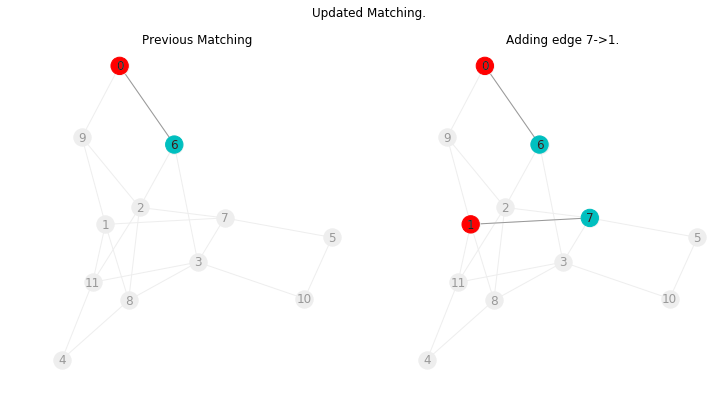
\includegraphics[width=\textwidth]{prim/5}
  \end{subfigure}
  \begin{subfigure}{0.49\textwidth}
    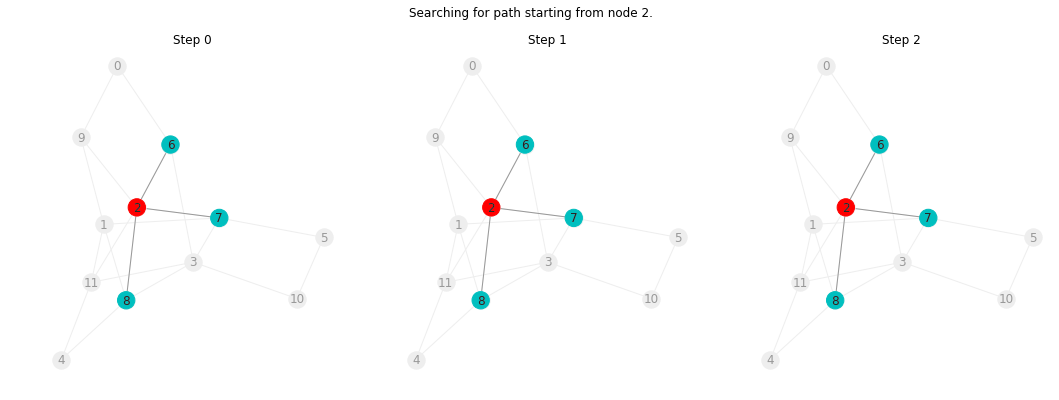
\includegraphics[width=\textwidth]{prim/6}
  \end{subfigure}
  \begin{subfigure}{0.49\textwidth}
    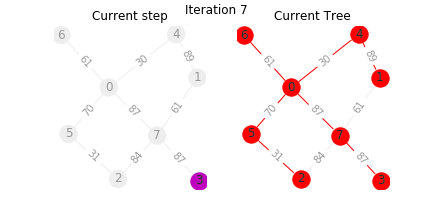
\includegraphics[width=\textwidth]{prim/7}
  \end{subfigure}
\end{figure}
\clearpage
\subsection{Validità degli algoritmi su MST}
\begin{definition}[Taglio]
  Dato un grafo \(\Gr \), chiamiamo \(\delta(A)\) con \(A \subseteq V\) l'insieme:
  \[
    \delta(A) = \crl{e \in E: \text{entrambi i vertici di \(e\) sono in \(A\)}}
  \]
  Questo insieme per qualche \(A\) è detto \textbf{taglio} di \(G\).
\end{definition}

\begin{theorem}[Tagli di grafi connessi]
  Un grafo \(\Gr \) è connesso se e solo se non esiste un insieme non vuoto \(A \subset V\) tale che:
  \[
    \delta(A) = \emptyset
  \]
\end{theorem}
\begin{proof}[Tagli di grafi connessi]
  È chiaro che se \(\delta(A) = \emptyset \), \(u \in A\) e \(v \not\in A\), allora non ci può essere un cammino da \(u\) a \(v\) e quindi se \(A \neq \emptyset \) e \(A \subset V\) allora G non è connesso.

  Dobbiamo dimostrare che, se \(G\) non è connesso, allora non esiste un tale set \(A\): scegliamo quindi due vertici \(u, v \in V\) tali che non esiste un cammino tra \(u\) a \(v\).

  Definiamo \(A\) come:
  \[
    A = \crl{w \in V: \text{esiste un cammino tra \(u\) a \(w\)}}
  \]
  Quindi \(u \in A\) e \(v \not\in A\), pertanto \(A \neq \emptyset \) e \(A \subset V\).

  Per dimostrare che \(\delta(A) = \emptyset \) procediamo per assurdo: supponiamo che \(p \in A\), \(q \not\in A\) e che \(e = \rnd{p,q} \in E\). Aggiungendo \(e\) a qualsiasi cammino da \(u\) a \(p\) si ottiene un cammino da \(u\) a \(q\), contraddicendo il fatto che \(q \not\in A\).
\end{proof}
\clearpage
\subsection{Diagramma della dimostrazione - Tagli di grafi connessi}
\begin{figure}
  \includegraphics[width=0.65\textwidth]{proofs/Tagli_di_grafi_connessi}
\end{figure}
\clearpage
\begin{definition}[Sottografo estensibile a MST]
  Un sottoinsieme di lati di \(\Gr \) \(A \subseteq E\) è estensibile a un MST se \(A\) è contenuto in un insieme di lati di qualche MST di \(G\).
\end{definition}
\begin{theorem}[Estensione a MST]
  Dato un grafo \(\Gr \), sia \(B \subseteq E\) un sottoinsieme estendibile a MST e \(e\) sia un lato a costo minimo di qualche taglio \(D\) tale che \(D \cap B = \emptyset \). Allora \(B \cup \crl{e}\) è estendibile ad un MST.
\end{theorem}
\begin{lemma}[Alberi ricoprenti]
  Sia \(H = \rnd{V, T}\) un albero ricoprente di \(G\), \(e = \rnd{v,w}\) un lato di \(G\) ma non di \(H\) e sia \(f\) un lato di un cammino semplice in \(T\) da \(v\) a \(w\). Allora il sottografo:
  \[
    H' = \rnd{V, \rnd{T \cup \crl{e}}\setminus \crl{f}}
  \]
  è un albero ricoprente di \(G\).
\end{lemma}
\begin{proof}[Estensione a MST]
  Sia \(H = \rnd{V, T}\) un MST tale che \(B \subseteq T\). Se \(e \in T\), allora abbiamo terminato il procedimento.

  Altrimenti, sia \(P\) un cammino semplice appartenente a \(H\) da \(v\) a \(w\), dove \(e = \rnd{v, w}\). Siccome non esiste nessun cammino in \(G\setminus D\) da \(v\) a \(w\), esiste un lato \(f \in P\) tale che \(f \in D\).

  Quindi \(c_f \geq c_e\), e per il lemma sugli alberi ricoprenti anche \(\rnd{V, \rnd{T \cup \crl{e}} \setminus \crl{f}}\) è un MST.

  Siccome \(D \cap B = \emptyset \), ne segue che \(f \not\in B\), pertanto \(B \cup \crl{e}\) è estendibile a un MST.
\end{proof}
\clearpage
\subsection{Diagramma della dimostrazione - Estensione a MST}
\begin{figure}
  \includegraphics[width=0.55\textwidth]{proofs/Estensione_a_MST}
\end{figure}
\clearpage
\section{MST e programmazione lineare}
\begin{theorem}[Teorema di Edmonds]
  Sia \(\bmxo\) il vettore caratteristico di un MST in rispetto ai costi \(\bmc \). ALlora \(\bmxo\) è una soluzione ottima del problema di programmazione lineare:
  \begin{align*}
    \min \bmct\bmx                                                                 \\
    x\rnd{\gamma(S)} & \leq \abs{S} -1 \quad \forall S \neq \emptyset, S \subset V \\
    x(E)             & = \abs{V} -1                                                \\
    x_e              & \geq 0                       \quad \forall e \in E
  \end{align*}
\end{theorem}
\begin{proof}[Teorema di Edmonds]
  Per un sottoinsieme di lati \(A\), sia \(k(A)\) il numero di componenti del sottografo \(\rnd{V, A}\) di \(G\). Prendiamo in considerazione una versione equivalente del problema proposto nel teorema:
  \begin{align*}
    \min \bmct\bmx                                           \\
    x\rnd{A} & \leq \abs{V} - k(A) \quad \forall A \subset E \\
    x(E)     & = \abs{V} -1                                  \\
    x_e      & \geq 0 \quad \forall e \in E
  \end{align*}
  Sia \(A \subseteq E\) e siano \(S_1, \ldots, S_k\) gli insiemi di vertici delle componenti del sottografo \(\rnd{V, A}\). Allora:
  \[
    x(A) \leq \sum_{i=1}^k x\rnd{\gamma\rnd{S_i}} \leq \sum_{i=1}^k \rnd{\abs{S_i}-1} = \abs{V} - k
  \]
  Procediamo ora a mostrare che \(\bmxo\) è la soluzione ottima del problema semplificato proposto e che è sufficiente perché ciò sia vero che essa è il vettore caratteristico di un albero ricoprente \(T\) generato dall'algoritmo di Kruskal.

  Mostriamo che \(\bmxo\) è ottimale mostrando che l'algoritmo di Kruskal può essere utilizzato per calcolare una soluzione ammissibile al problema PL duale che soddisfa gli scarti complementari con \(\bmxo\). Riscrivendo la funzione obbiettivo del problema primale come \(\max -\bmct\bmx \), il duale risulta:
  \begin{align*}
    \min \sum_{A \subseteq W} \rnd{\abs{V} - k(A)}\bmy_A           \\
    \sum \rnd{\bmy_a: e \in A} & \geq -c_e, \quad \forall e \in E  \\
    \bmy_A                     & \geq 0, \quad \forall A \subset E
  \end{align*}
  Sia \(e_1, \ldots, e_m\) l'ordine con cui l'algoritmo di Kruskal considera i lati. Sia \(R_i = \crl{e_1, \ldots, e_i}, \forall i \in \N \cap \sqr{1, m}\).

  Sia \(\bmy_A^o=0\) a meno che \(\exists i: A = R_i\), e assegniamo \(\bmy^o_{R_i} = c_{e_{i+1}} - c_{e_{i}} \forall i \in \N \cap \sqr{1, m-1}\). Infine assegniamo \(\bmy^o_{R_m} = -c_{e_m}\).

  Segue dall'ordine dei lati considerati dall'algoritmo che \(\bmy^o_A \geq 0\) se \(A\neq E\). Considerando ora il vincolo a sommatoria del problema, dove \(e=e_i\) abbiamo:
  \[
    \sum_{\bmy^o_A: e \in A} = \sum_{j=i}^m \bmy^o_{R_j} = \sum_{j=i}^{m-1}\rnd{c_{e_{i+1}}-c_{e_i}} - c_{e_m} = -c_{e_i} = -c_e
  \]
  In altre parole, tutte le disuguaglianze considerate valgono come uguaglianze, pertanto la soluzione \(\bmy^o\) è ammissibile e rispetta le condizioni degli scarti complementari: rimane solo una condizione da verificare, cioè se:
  \[
    \bmy^o_A > 0 \Rightarrow \bm\bmxo \text{ soddisfa le condizioni degli scarti complementari.}
  \]
  Per verificare questo, sappiamo che \(\exists i: A = R_i\). Se i vincoli del problema primale non soddisfano le condizioni degli scarti complementari per \(R_i\), allora esiste qualche lato di \(R_i\) la cui aggiunta a \(T\cap R_i\) porterebbe a ridurre il numero di componenti di \(\rnd{V, T \cap R_i}\). Ma un tale lato avrebbe termini in due componenti diverse di \(\rnd{V, R_i \cup T}\), e quindi sarebbe stato aggiunto a \(T\) dall'algoritmo di Kruskal.

  Per cui, \(\bm\bmxo\) e \(\bmy^o\) soddisfano le condizioni degli scarti complementari. Ne segue che \(\bm\bmxo\) è la soluzione ottima del problema di PL.
\end{proof}
\clearpage
\subsection{Diagramma della dimostrazione - Teorema di Edmonds}
\begin{figure}
  \includegraphics[width=\textwidth]{proofs/H_Legame_tra_MST_e_PL}
\end{figure}
\end{document}